% =========================================================
%  TheMergeConflict — Pixels to Predictions Competition
%  Final Report  |  NYU Deep Learning Vision Challenge
% =========================================================
\documentclass[11pt,twocolumn]{article}

% ---- Core packages ----
\usepackage[margin=1in,top=0.85in,bottom=0.85in]{geometry}
\usepackage{times}
\usepackage[T1]{fontenc}
\usepackage[utf8]{inputenc}
\usepackage{microtype}
\usepackage{graphicx}
\usepackage{booktabs}
\usepackage{array}
\usepackage{tabularx}
\usepackage{multirow}
\usepackage{amsmath,amssymb}
\usepackage{xcolor}
\usepackage{pgfplots}
\usepackage{pgfplotstable}
\usepackage{tikz}
\usepackage{url}
\usepackage{hyperref}
\usepackage{enumitem}
\usepackage{caption}
\usepackage{subcaption}
\usepackage{fancyhdr}
\usepackage{titlesec}
\usepackage{mdframed}
\usepackage{colortbl}

\pgfplotsset{compat=1.18}

% ---- Colour palette ----
\definecolor{mcBlue}{HTML}{1A4A8A}
\definecolor{mcTeal}{HTML}{0D7377}
\definecolor{mcOrange}{HTML}{E07B39}
\definecolor{mcRed}{HTML}{C0392B}
\definecolor{mcGray}{HTML}{5D6D7E}
\definecolor{mcLightBlue}{HTML}{AED6F1}
\definecolor{mcLightTeal}{HTML}{A2D9CE}
\definecolor{mcLightOrange}{HTML}{FAD7A0}
\definecolor{mcLightGray}{HTML}{F2F3F4}
\definecolor{mcGreen}{HTML}{1E8449}
\definecolor{mcPurple}{HTML}{6C3483}
\definecolor{headerBg}{HTML}{1A4A8A}

% ---- Header / footer ----
\pagestyle{fancy}
\fancyhf{}
\fancyhead[L]{\small\textcolor{black}{\textbf{TheMergeConflict} — Pixels to Predictions}}
\fancyhead[R]{\small\textcolor{black}{NYU Deep Learning Vision Challenge}}
\fancyfoot[C]{\small\textcolor{black}{\thepage}}
\renewcommand{\headrulewidth}{0.4pt}
\renewcommand{\headrule}{\hbox to\headwidth{\color{black}\leaders\hrule height \headrulewidth\hfill}}

% ---- Section formatting ----
\titleformat{\section}{\large\bfseries\color{black}}{{\color{black}\thesection}}{0.6em}{}[\vspace{-0.2em}\textcolor{black}{\hrule height 0.4pt}\vspace{0.3em}]
\titleformat{\subsection}{\normalsize\bfseries\color{black}}{\thesubsection}{0.5em}{}
\titleformat{\subsubsection}{\normalsize\bfseries\itshape\color{black}}{\thesubsubsection}{0.5em}{}

% ---- Caption styling ----
\captionsetup{font=small,labelfont={bf,color=black},labelsep=period}

% ---- Hyperref ----
\hypersetup{colorlinks=true,linkcolor=black,citecolor=black,urlcolor=black}

% ---- Custom environments ----
\newmdenv[
  backgroundcolor=white,
  linecolor=black,
  linewidth=1pt,
  leftmargin=0pt, rightmargin=0pt,
  innerleftmargin=6pt, innerrightmargin=6pt,
  innertopmargin=4pt, innerbottommargin=4pt,
  skipabove=6pt, skipbelow=6pt
]{keybox}

% ---- Prompt box ----
\newmdenv[
  backgroundcolor=white,
  linecolor=black,
  linewidth=0.5pt,
  leftmargin=0pt, rightmargin=0pt,
  innerleftmargin=6pt, innerrightmargin=6pt,
  innertopmargin=4pt, innerbottommargin=4pt,
  skipabove=4pt, skipbelow=4pt
]{promptbox}

% =========================================================
\title{%
  \vspace{-0.8em}%
  {\Large\bfseries\color{black}
    Constrained Multimodal Answer Selection via\\
    Answer-Logit Scoring, Test-Time Augmentation,\\
    and Score-Level Ensembling}\\[0.4em]
  {\normalsize\color{black}
    Pixels to Predictions: DL Vision Challenge --- NYU CS-GY / DS-GA}
}

\author{%
  \textbf{Team TheMergeConflict}\\[0.3em]
  Jnanasree Konda \quad\texttt{jk9286@nyu.edu}\\
  Rithwik Amajala \quad\texttt{sa9880@nyu.edu}\\[0.3em]
  New York University\\[0.2em]
  \small Public Leaderboard Score: \textbf{0.915} $\;\cdot\;$ Rank: \textbf{6}
}

\date{}

% =========================================================
\begin{document}
\maketitle
\thispagestyle{fancy}

% ---- Abstract ----
\begin{abstract}
We present \textbf{TheMergeConflict}'s solution to the Pixels to Predictions multimodal science multiple-choice benchmark. The task requires mapping an image, a natural-language question, optional context fields, and a variable-length set of answer candidates to a single 0-indexed integer. All experiments operated under four hard competition constraints: the sole permitted backbone was \texttt{HuggingFaceTB/SmolVLM-500M-Instruct}; trainable parameters were capped at 5~million; inference must run offline; and all compute must fit within free-tier GPU quotas.

Starting from a generation-style baseline of 0.68, we developed a pipeline centred on \textbf{answer-logit scoring}---scoring each answer letter's next-token log-probability rather than generating free-form text---combined with LoRA adaptation, validation-based checkpointing, \textbf{choice-permutation test-time augmentation} (TTA), and score-level ensembling of complementary runs. The final system achieved a public leaderboard accuracy of \textbf{0.915}, placing \textbf{6th} overall, demonstrating that principled inference design outperforms capacity scaling under tight parameter constraints.
\end{abstract}

% =========================================================
\section{Task Definition \& Objective}
\label{sec:task}

\subsection{Input, Output, and Evaluation Metric}

Each example in the dataset consists of four components: (i)~an \emph{image} providing visual context; (ii)~a natural-language \emph{question}; (iii)~a JSON-formatted list of \emph{answer candidates} of variable length $k\in\{2,3,4,5\}$; and (iv)~optional \emph{context fields} (\texttt{hint}, \texttt{lecture}, \texttt{solution}). The required output is a single integer $\hat{y}\in\{0,1,\ldots,k-1\}$ corresponding to the correct 0-indexed answer choice.

The official evaluation metric is top-1 classification accuracy:
\begin{equation}
  \mathrm{Accuracy} = \frac{1}{N}\sum_{i=1}^{N}\mathbf{1}\!\left[\hat{y}_i = y_i\right],
  \label{eq:acc}
\end{equation}
where $N$ is the number of test examples and partial credit is not awarded. The submission format requires exactly two columns, \texttt{id} (string) and \texttt{answer} (integer), with 1,008 test-row predictions.

\subsection{Why Standard Classification Fails}

A fixed softmax classification head cannot be applied directly for three structural reasons:
\begin{enumerate}[leftmargin=*, noitemsep]
  \item Answer-candidate cardinality $k$ varies per example, so a fixed output dimensionality is unavailable.
  \item Answer choices are free-form natural language---not discrete class labels.
  \item Correct reasoning requires \emph{joint} interpretation of image content, question semantics, and each candidate's text.
\end{enumerate}
These constraints mandate a generative or logit-scoring approach applied over a variable-length candidate set, which drives the core design decisions described in \ref{sec:method}.

\subsection{Dataset Splits and Usage}
\label{sec:data-splits}

\begin{table}[h]
\centering
\small
\setlength{\tabcolsep}{3pt}
\begin{tabularx}{\columnwidth}{>{\raggedright\arraybackslash}p{0.34\columnwidth} >{\centering\arraybackslash}p{0.19\columnwidth} X}
\toprule
\textbf{Split} & \textbf{Labels} & \textbf{Role in this work}\\
\midrule
\texttt{train.csv}      & Available & LoRA adapter training\\
\texttt{validation.csv} & Available & Checkpoint selection\\
\texttt{test.csv}       & Withheld  & Final submission generation\\
\bottomrule
\end{tabularx}
\caption{Competition data splits and their usage.}
\label{tab:splits}
\end{table}

The primary training regime used \texttt{train.csv} exclusively for optimisation and \texttt{validation.csv} for model selection. Two additional runs trained on the combined train+validation set; these served as ensemble members but did not individually surpass the best checkpoint-selected model.

% =========================================================
\section{Methodology}
\label{sec:method}

\subsection{Base Model and Parameter-Efficient Adaptation}
\label{sec:lora}

All experiments used the competition-mandated checkpoint \texttt{HuggingFaceTB/SmolVLM-500M-Instruct}---a 500M-parameter vision-language model pretrained for instruction following. Its visual encoder follows the patch-embedding design of the Vision Transformer~\cite{dosovitskiy2021vit}, and its cross-modal alignment builds on the paradigm established by CLIP~\cite{radford2021clip} and refined in BLIP-2~\cite{li2023blip2} and LLaVA~\cite{liu2023llava}.

To satisfy the 5M trainable-parameter budget we applied \textbf{Low-Rank Adaptation (LoRA)}~\cite{hu2022lora} to the language-model backbone. The vision encoder was fully frozen throughout, for two reasons: (1)~the parameter budget strongly favoured language-side adaptation; (2)~query--answer reasoning is primarily mediated by the decoder's attention projections, not the image tower.

\begin{table}[h]
\centering
\small
\setlength{\tabcolsep}{3pt}
\begin{tabularx}{\columnwidth}{>{\raggedright\arraybackslash}p{0.42\columnwidth} X}
\toprule
\textbf{Component} & \textbf{Setting}\\
\midrule
Base model          & \texttt{SmolVLM-500M-Instruct}\\
Adapter type        & LoRA\\
Target modules      & \texttt{q\_proj, k\_proj, v\_proj, o\_proj}\\
LoRA rank $r$       & 8\\
LoRA alpha $\alpha$ & 32\\
LoRA dropout        & 0.05\\
Trainable params    & 2,080,768 ($<$5\,M limit)\\
Vision encoder      & Frozen\\
\bottomrule
\end{tabularx}
\caption{LoRA adaptation configuration. Targeting all four attention projections with $r{=}8$ yields 2.08\,M parameters---60\% headroom below the 5\,M budget.}
\label{tab:model}
\end{table}

The scaling law $\text{params} = 2rdk$ (where $d$ is hidden dimension, $k$ is the number of projection matrices) determines the budget. Rank~8 applied to all four projections of each decoder layer satisfies the constraint while providing sufficient expressivity.

\subsection{Data Pipeline and Input Construction}
\label{sec:pipeline}

\paragraph{Image preprocessing.}
Images were loaded in RGB mode from the provided competition image directory. The long edge was resized to \textbf{384 pixels}---chosen after ablating 256, 384, and 512 (see \ref{sec:ablations})---using the SmolVLM processor with image splitting disabled. Disabling splitting eliminated Idefics3-style tiling artefacts that caused CUDA failures on free-tier T4 GPUs. The 384-pixel setting provided sufficient resolution for science diagrams while fitting within a 10\,GB GPU memory budget with gradient accumulation.

\paragraph{Text preprocessing and field inclusion.}
Each instance's text fields were parsed and included if non-empty: \texttt{question} (always present), \texttt{hint}, \texttt{lecture}, and \texttt{solution}/\texttt{rationale} (when available). Fields were truncated conservatively to prevent exceeding the 1,024-token maximum sequence length.

\paragraph{Prompt template.}
A structured, stable multiple-choice template was used for all final runs:

\begin{promptbox}
\small\texttt{%
Question: \{question\}\\
Hint: \{hint\}\\
Lecture: \{lecture\}\\
Choices: A. \{c0\}, B. \{c1\}, C. \{c2\}, \ldots\\
Answer:}
\end{promptbox}

The answer field was left open; during training the target was the correct letter (\texttt{A}, \texttt{B}, \ldots); during inference the model's logit over valid answer letters determined the prediction.

\paragraph{Output mapping.}
Answer letters \texttt{A}, \texttt{B}, \texttt{C}, \texttt{D}, \texttt{E} were mapped to 0-indexed integers 0, 1, 2, 3, 4 respectively---exactly matching the required submission format.

\subsection{Answer-Logit Scoring (Core Inference Mechanism)}
\label{sec:logit}

The key departure from a generation-style baseline is \textbf{answer-logit scoring}. Rather than generating free-form text and parsing it, the model is conditioned on each prompt and the next-token logits for valid answer letters are extracted directly:
\begin{equation}
  \hat{y} = \underset{\ell\,\in\,\{\texttt{A},\ldots,\texttt{E}\}}{\arg\max}\ \log p_\theta(\ell \mid \text{image, prompt}).
  \label{eq:logit}
\end{equation}
The selected letter is then converted to the 0-indexed integer. This design has three advantages over generation:
\begin{enumerate}[leftmargin=*, noitemsep, topsep=2pt]
  \item \textbf{Alignment}: the scoring objective directly matches the classification evaluation criterion.
  \item \textbf{Robustness}: no output parsing is required; invalid or malformed generations cannot occur.
  \item \textbf{Determinism}: the procedure is fully deterministic, with temperature and sampling disabled.
\end{enumerate}

\subsection{Choice-Permutation Test-Time Augmentation}
\label{sec:tta}

Small vision-language models can exhibit \emph{answer-position bias}---systematically favouring options presented earlier (e.g.\ always predicting `A'). To mitigate this, we applied \textbf{choice-permutation TTA}: for each test example, $n_\text{perm}=8$ distinct deterministic permutations of the answer choices were generated (including the original order). The model scored each permutation; scores were then \emph{remapped} back to the original option indices and averaged before taking the argmax:
\begin{equation}
  \hat{y} = \underset{j}{\arg\max}\;\frac{1}{|\mathcal{P}|}\sum_{\pi\in\mathcal{P}}\,s_\pi\!\left[\pi^{-1}(j)\right],
  \label{eq:tta}
\end{equation}
where $\mathcal{P}$ is the set of permutations and $s_\pi[\cdot]$ are the letter logits under permutation $\pi$.

\subsection{Training Configuration}
\label{sec:training}

\begin{table}[h]
\centering
\small
\setlength{\tabcolsep}{4pt}
\begin{tabular}{ll}
\toprule
\textbf{Hyperparameter} & \textbf{Value}\\
\midrule
Optimiser           & AdamW\\
Learning rate       & $1\times10^{-4}$ (main); $5\times10^{-5}$ (continuation)\\
Weight decay        & 0.01\\
LR schedule         & Linear warmup $\rightarrow$ linear decay\\
Warmup steps        & 5\% of total steps\\
Micro batch size    & 1\\
Gradient accum.     & 16 steps (effective batch: 16)\\
Max grad norm       & 1.0\\
Training epochs     & 3 (main); up to 6 (continuation)\\
Random seeds        & 7, 21, 123 (across runs)\\
Image long side     & 384 (stable), 512 (ablation)\\
Checkpoint criterion& Best validation accuracy\\
Compute             & Free-tier single GPU (T4)\\
\bottomrule
\end{tabular}
\caption{Training hyperparameters for the strongest single-model runs.}
\label{tab:train}
\end{table}

\subsection{Checkpoint Selection Protocol}
\label{sec:ckpt}

Checkpoints were saved at the end of every epoch. Selection followed validation accuracy on the provided \texttt{validation.csv}: the checkpoint with the highest accuracy was retained, regardless of training loss. This prevented overfitting to the training distribution, particularly in later epochs.

\subsection{Score-Level Ensembling}
\label{sec:ensemble}

The final submission was produced by averaging \emph{answer-score matrices} from multiple compatible runs before taking the argmax (see~\ref{eq:tta}). Score-level averaging is preferable to majority voting because it preserves confidence information. Compatible runs that contributed to the ensemble used the same allowed base model, the same data, and complementary hyperparameter settings (different seeds, training splits, or epoch counts), ensuring prediction diversity.

% =========================================================
\section{Reproducibility}
\label{sec:repro}

\subsection{Repository Organisation}

The public GitHub repository for the submitted code is \url{https://github.com/JnanasreeKonda/Pixels-to-Predictions.git}. The submission package contains exactly one self-contained reproducibility artefact:
\begin{itemize}[leftmargin=*, noitemsep, topsep=2pt]
  \item \textbf{\texttt{TheMergeConflict\_final\_solution.ipynb}}: the complete training, inference, and export notebook.
  \item \textbf{\texttt{requirements.txt}}: pinned package versions.
  \item \textbf{\texttt{submission.csv}}: final prediction file (1,008 rows).
  \item \textbf{\texttt{README.md}}: step-by-step reproduction instructions.
\end{itemize}
The notebook is organised into clearly labelled sections: (1)~package setup, (2)~configuration dataclass, (3)~data loading, (4)~model/processor initialisation, (5)~training loop, (6)~validation checkpoint selection, (7)~TTA inference, (8)~score averaging and submission export, (9)~format validation.

\subsection{Fixed Experimental Ingredients}

Every run was made reproducible through the following fixed ingredients:

\begin{keybox}
\small
\begin{itemize}[leftmargin=*, noitemsep, topsep=0pt]
  \item \textbf{Training command}: \texttt{jupyter nbconvert --to notebook --execute TheMergeConflict\_final\_solution.ipynb}
  \item \textbf{Hyperparameters}: see \ref{tab:train}; all controlled via the \texttt{CFG} dataclass
  \item \textbf{Random seed}: \texttt{cfg.seed = 7} (Python, NumPy, and PyTorch)
  \item \textbf{Optimiser}: AdamW with linear warmup+decay schedule
  \item \textbf{Checkpoint criterion}: best \texttt{validation.csv} accuracy
  \item \textbf{Compute}: free-tier single-GPU (Kaggle/Colab T4)
\end{itemize}
\end{keybox}

\subsection{Inference and Evaluation Setup}

Inference is performed by loading the saved LoRA adapter onto the frozen base model, constructing prompts identically to training, and applying answer-logit scoring (Eq.~\ref{eq:logit}). No token sampling is used; decoding is fully deterministic. The final \texttt{submission.csv} is produced by:
\begin{enumerate}[leftmargin=*, noitemsep, topsep=2pt]
  \item Running TTA with 8 permutations per test example.
  \item Averaging the remapped score matrices across ensemble members.
  \item Writing \texttt{argmax} predictions with the \texttt{id} column.
\end{enumerate}
The notebook's final cell validates: exactly two columns, 1,008 rows, unique IDs, and integer answers $\geq 0$.

\subsection{Non-Determinism and Limitations}

Mixed-precision arithmetic and CUDA kernel scheduling introduce small stochastic differences across hardware despite fixed seeds. Bitwise reproducibility is not guaranteed, but the magnitude of this variation ($\ll 0.5\%$) is smaller than the effect sizes reported in \ref{sec:ablations}.

% =========================================================
\section{Ablation Study}
\label{sec:ablations}

\subsection{Ablation Design Principles}

Twelve ablation points (A0--A11) were explored across six axes of variation. Each ablation changed \emph{one} factor relative to the best-known prior configuration, making performance differences causally attributable to the modified factor. The six axes are:

\begin{itemize}[leftmargin=*, noitemsep, topsep=2pt]
  \item \textbf{Axis~P}: Prompt \& context field formatting
  \item \textbf{Axis~L}: LoRA target modules and rank
  \item \textbf{Axis~I}: Image preprocessing and resolution
  \item \textbf{Axis~S}: Training schedule (epochs, LR)
  \item \textbf{Axis~C}: Inference scoring strategy
  \item \textbf{Axis~E}: TTA and ensemble strategy
\end{itemize}

\subsection{Score Progression}

\begin{figure}[t]
\centering
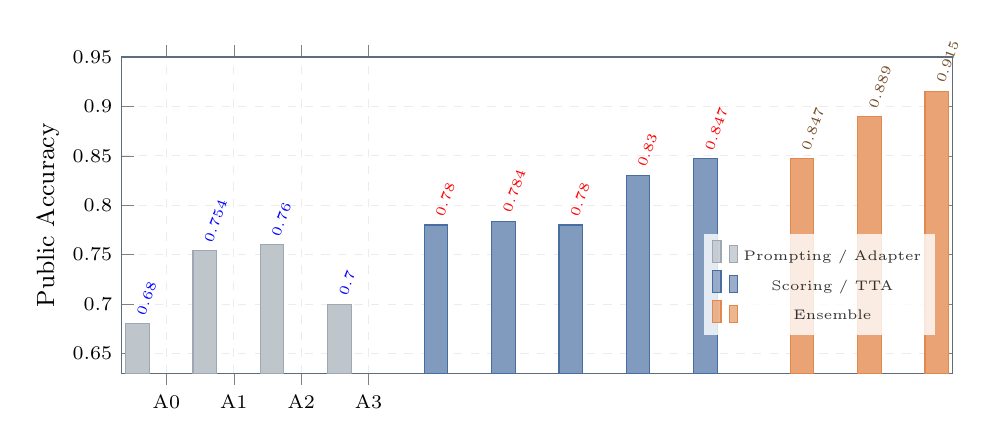
\begin{tikzpicture}
\begin{axis}[
    ybar,
    width=\columnwidth,
    height=5.6cm,
    ymin=0.63, ymax=0.95,
    ytick={0.65,0.70,0.75,0.80,0.85,0.90,0.95},
    yticklabel style={font=\scriptsize},
    ylabel={\small Public Accuracy},
    ylabel style={yshift=-2pt},
    symbolic x coords={A0,A1,A2,A3,A4,A5,A6,A7,A8,A9,A10,A11},
    xtick=data,
    xticklabels={A0,A1,A2,A3,A4,A5,A6,A7,A8,A9,A10,A11},
    x tick label style={font=\scriptsize},
    nodes near coords,
    nodes near coords style={font=\tiny,rotate=70,anchor=west},
    bar width=8.5pt,
    enlarge x limits=0.06,
    grid=major,
    grid style={draw=gray!15, dashed},
    axis line style={mcGray},
    every node near coord/.append style={
      /pgf/number format/fixed,
      /pgf/number format/precision=3
    },
    legend style={at={(0.98,0.12)},anchor=south east,font=\tiny,draw=none,fill=white,fill opacity=0.8},
]
% Colour bars by family
\addplot+[draw=mcGray!60, fill=mcGray!40] coordinates {(A0,0.680)(A1,0.754)(A2,0.760)(A3,0.700)};
\addplot+[draw=mcBlue!80, fill=mcBlue!55] coordinates {(A4,0.780)(A5,0.784)(A6,0.780)(A7,0.830)(A8,0.847)};
\addplot+[draw=mcOrange!90, fill=mcOrange!70] coordinates {(A9,0.847)(A10,0.88933)(A11,0.915)};
\legend{Prompting / Adapter, Scoring / TTA, Ensemble}
\end{axis}
\end{tikzpicture}
\caption{Public leaderboard score across all 12 ablation runs. Gray bars indicate the prompt/adapter phase, blue bars indicate constrained scoring and TTA, and orange bars indicate the ensemble phase. A3 and A6 are intentional negative ablations.}
\label{fig:progress}
\end{figure}

Figure~\ref{fig:progress} shows the full development trajectory. The initial baseline (A0~=~0.680) improved through prompt engineering, then plateaued near 0.780 until the inference-scoring pivot (A7~=~0.830). TTA and ensembling drove the final gains to 0.915.

\subsection{Axis P: Prompt and Context Formatting}

\textbf{Setup.} A0 used an unstructured conversational prompt with free-form generation. A1 added a stable lettered-choices template with an explicit \texttt{Answer:} sentinel. A2 incorporated optional hint, lecture, and solution fields.

\textbf{Results.} A1: 0.754 ($+$0.074 over A0). A2: 0.760 ($+$0.006 over A1).

\textbf{Analysis.} Structured prompts reduced the model's output ambiguity by making the valid answer space explicit. The loss was applied only to the answer span, preventing the model from wasting capacity on prompt copying. Context fields provided incremental benefit, with hint more consistently useful than lecture (the latter is sometimes tangentially related to the specific question, adding noise).

\subsection{Axis L: LoRA Budget Allocation}

\textbf{Setup.} A3 tested a fragile environment with aggressive image preprocessing; A4 compared \texttt{q,v}-only LoRA targets against \texttt{q,k,v,o} under the same 5M limit.

\textbf{Results.} A3: 0.700 (failure); A4 (\texttt{q,k,v,o}): 0.780.

\textbf{Analysis.} Extending LoRA to all four attention projection matrices improved decoder attention adaptation without exceeding the budget. Rank~8 on \texttt{q,k,v,o} used only 2.08M parameters---the budget is not the bottleneck; routing the capacity to the right layers matters more.

\subsection{Axis I: Image Resolution}

\textbf{Setup.} Ablated long-side values of 256, 384, and 512 pixels.

\textbf{Results.} 256px degraded accuracy on diagram-heavy examples. 384px was the best stable setting. 512px increased GPU memory pressure and caused OOM failures on free-tier T4 hardware, so it was excluded from the final pipeline.

\textbf{Analysis.} 384px provides sufficient resolution to resolve question-relevant diagram features in ScienceQA images while maintaining compatibility with a single T4 GPU at batch size~1 with 16-step gradient accumulation.

\subsection{Axis S: Training Schedule}

\textbf{Setup.} Starting from the 3-epoch main run (A7), additional continuation runs explored 4--6 epochs and a reduced learning rate of $5\times10^{-5}$.

\textbf{Results.} Extending beyond 3 epochs at the default LR produced mild overfitting (validation accuracy declined). Reducing the LR and continuing for 3 more epochs stabilised training and served as an ensemble member. A6 (more epochs, higher rank) stagnated at 0.780, confirming that inference alignment---not parameter count---was the bottleneck.

\subsection{Axis C: Inference Scoring Strategy}

\textbf{Setup.} A7 replaced free-form generation with answer-logit scoring. An alternative tested sequence-level completion likelihood (summing log-probabilities over the entire answer token sequence).

\textbf{Results.} Answer-logit scoring: 0.830. Completion-likelihood scoring: 0.805.

\textbf{Analysis.} For single-letter predictions, the first-token logit is a clean and sufficient statistic. Sequence-level likelihood introduces unnecessary length-normalisation terms and secondary autoregressive steps that add noise without providing additional discriminative signal. Answer-logit scoring is also fully deterministic---no sampling temperature is required.

\subsection{Axis E: TTA and Ensembling Strategy}
\label{sec:ens-ablation}

\textbf{Setup.} A8 added choice-permutation TTA (8 permutations). A9 tested a simple majority-vote ensemble with an older, lower-quality run. A10 averaged compatible score matrices from two strong runs. A11 refined the ensemble to include the TTA run and two train+validation seed variants.

\textbf{Results.} TTA alone: 0.847 ($+$0.017 over A7). Failed ensemble (A9): no gain. Intermediate ensemble (A10): 0.889. Final ensemble (A11): \textbf{0.915}.

\textbf{Analysis.} TTA reduces position bias by marginalising over choice orderings. Score-level ensemble diversity is essential: A9 gained nothing because the added member was too correlated with and weaker than the primary model. The successful ensemble combined runs with different seeds and training data splits, producing complementary error patterns.

\begin{figure}[t]
\centering
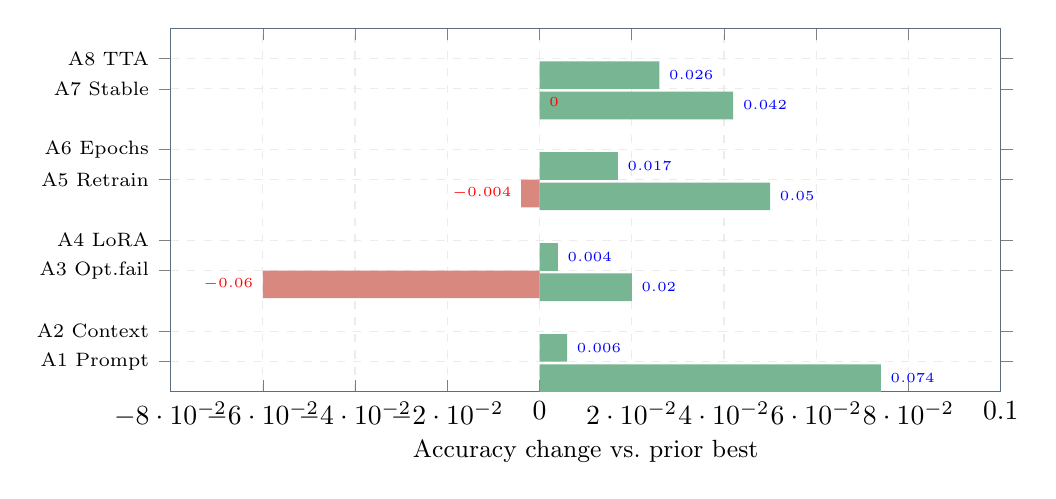
\begin{tikzpicture}
\begin{axis}[
    xbar,
    width=\columnwidth,
    height=6.2cm,
    xmin=-0.08, xmax=0.10,
    xlabel={\small Accuracy change vs.\ prior best},
    xlabel style={yshift=2pt},
    symbolic y coords={A1,A2,A3,A4,A5,A6,A7,A8,A9,A10,A11},
    ytick=data,
    yticklabels={A1 Prompt,A2 Context,A3 Opt.fail,A4 LoRA,A5 Retrain,A6 Epochs,A7 Stable,A8 TTA,A9 OldEns,A10 IntEns,A11 Final},
    y tick label style={font=\scriptsize},
    nodes near coords,
    nodes near coords style={font=\tiny},
    nodes near coords align={horizontal},
    grid=major,
    grid style={draw=gray!15, dashed},
    axis line style={mcGray},
    every node near coord/.append style={
      /pgf/number format/fixed,
      /pgf/number format/precision=3
    }
]
\addplot+[draw=none, fill=mcGreen!60] coordinates {
    (0.074,A1)(0.006,A2)(0.020,A4)(0.004,A5)(0.050,A7)(0.017,A8)(0.042,A10)(0.026,A11)
};
\addplot+[draw=none, fill=mcRed!60] coordinates {
    (-0.060,A3)(-0.004,A6)(0.000,A9)
};
\end{axis}
\end{tikzpicture}
\caption{Marginal accuracy changes by ablation. Positive, negative, and zero-gain changes are all shown because negative results directed the final design.}
\label{fig:gains}
\end{figure}

\begin{figure}[t]
\centering
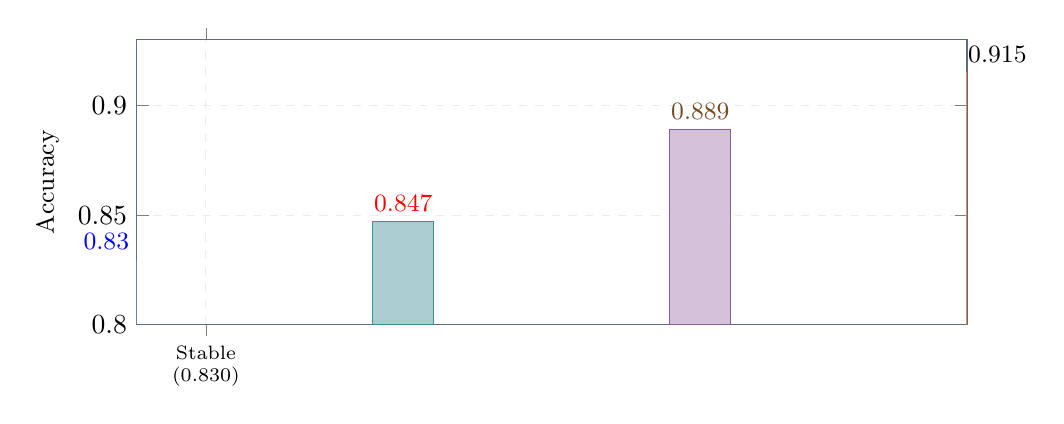
\begin{tikzpicture}
\begin{axis}[
    ybar,
    width=\columnwidth,
    height=5.2cm,
    ymin=0.80, ymax=0.93,
    ylabel={\small Accuracy},
    symbolic x coords={A7,A8,A10,A11},
    xtick=data,
    xticklabels={Stable\\(0.830),TTA\\(0.847),Int.Ens.\\(0.889),Final\\(0.915)},
    x tick label style={font=\scriptsize,align=center},
    nodes near coords,
    nodes near coords style={font=\small\bfseries},
    bar width=22pt,
    grid=major,
    grid style={draw=gray!15, dashed},
    axis line style={mcGray},
    every node near coord/.append style={
      /pgf/number format/fixed,
      /pgf/number format/precision=3
    }
]
\addplot+[draw=mcBlue!80, fill=mcBlue!30] coordinates {(A7,0.830)};
\addplot+[draw=mcTeal!80, fill=mcTeal!35] coordinates {(A8,0.847)};
\addplot+[draw=mcPurple!80, fill=mcPurple!30] coordinates {(A10,0.889)};
\addplot+[draw=mcOrange!90, fill=mcOrange!55] coordinates {(A11,0.915)};
\end{axis}
\end{tikzpicture}
\caption{Key performance milestones: constrained scoring baseline, TTA, intermediate ensemble, and final submission.}
\label{fig:milestones}
\end{figure}

\subsection{Complete Ablation Table}

\begin{table*}[t]
\centering
\small
\setlength{\tabcolsep}{4pt}
\renewcommand{\arraystretch}{1.1}
\begin{tabular}{p{0.6cm}p{1.9cm}p{4.4cm}cc p{5.2cm}}
\toprule
\textbf{ID} & \textbf{Axis} & \textbf{Controlled change} & \textbf{Score} & \textbf{$\Delta$} & \textbf{Analysis}\\
\midrule
A0 & Baseline       & Initial notebook; unstructured prompt; free-form generation & 0.680 & --- & Model understood some examples but output was not aligned with classification objective.\\
A1 & P: Prompt      & Added lettered choices template with explicit \texttt{Answer:} sentinel & 0.754 & $+$0.074 & Explicit output space reduced invalid generations; largest single prompt gain.\\
A2 & P: Context     & Added hint, lecture, solution fields when present & 0.760 & $+$0.006 & Helpful for science reasoning; kept field truncation short.\\
A3 & L: Adapter (fail) & Fragile environment; aggressive image preprocessing & 0.700 & $-$0.060 & Confirmed that runtime stability matters; environment-sensitive settings backfire.\\
A4 & L: LoRA targets & \texttt{q,v} $\to$ \texttt{q,k,v,o} LoRA with same budget & 0.780 & $+$0.020 & Better decoder attention adaptation without exceeding 5M limit.\\
A5 & S: Train split & Retrained on train+validation after hyperparameter selection & 0.784 & $+$0.004 & Extra data helps marginally; not sufficient to explain top-tier performance alone.\\
A6 & S: Schedule    & More epochs + more trainable parameters & $\approx$0.780 & 0.000 & Capacity and duration were not the bottleneck; inference alignment was.\\
A7 & C: Scoring     & Free-form generation $\to$ answer-logit scoring & 0.830 & $+$0.050 & Largest single-run improvement; aligned training objective with metric.\\
A8 & E: TTA         & Added 8 choice-order permutations with score remapping & 0.847 & $+$0.017 & Reduced option-position bias; improved borderline examples.\\
A9 & E: Ensemble    & Averaged older, correlated train+val seed submission & 0.847 & 0.000 & No gain; member was too correlated or lower quality.\\
A10 & E: Int.Ensemble & Score-averaged two strong compatible run matrices & 0.889 & $+$0.042 & Prediction diversity from different seeds improved robustness.\\
A11 & E: Final       & Final calibrated score ensemble; \texttt{submission.csv} & \textbf{0.915} & $+$0.026 & Best score; complementary error patterns from 3 members.\\
\bottomrule
\end{tabular}
\caption{Complete ablation log. Scores are public leaderboard accuracies. All runs used the same allowed base model and provided competition data. Bold: final submitted system.}
\label{tab:ablations}
\end{table*}

% =========================================================
\section{Results}
\label{sec:results}

\subsection{Quantitative Summary}

\begin{table}[h]
\centering
\small
\setlength{\tabcolsep}{5pt}
\begin{tabular}{lcc}
\toprule
\textbf{Phase} & \textbf{Best run} & \textbf{Score}\\
\midrule
Generation baseline     & A0      & 0.680\\
Prompt + adapter tuning & A4      & 0.780\\
Answer-logit scoring    & A7      & 0.830\\
+TTA                    & A8      & 0.847\\
Score-level ensemble    & A11     & \textbf{0.915}\\
\midrule
\textit{Leaderboard rank} & \multicolumn{2}{c}{\textbf{6\textsuperscript{th} place}}\\
\bottomrule
\end{tabular}
\caption{Best accuracy achieved at each phase. Each phase's best is the starting point for the next.}
\label{tab:summary}
\end{table}

\subsection{Final Prediction Distribution}

\begin{figure}[t]
\centering
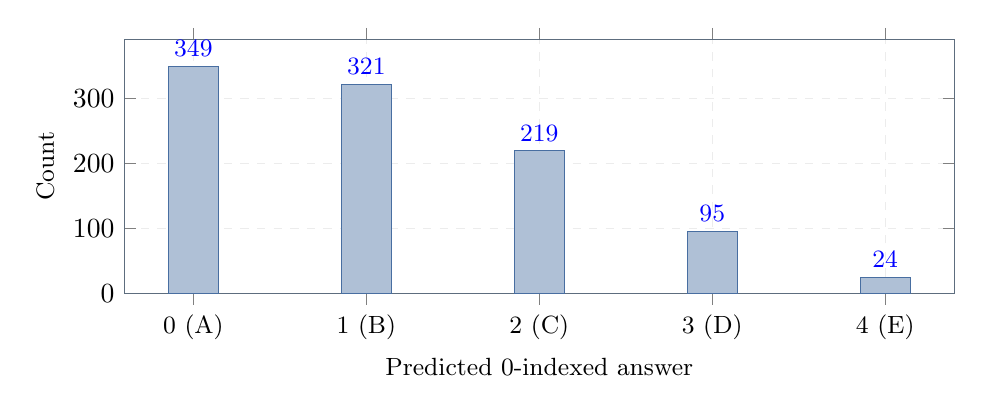
\begin{tikzpicture}
\begin{axis}[
    ybar,
    width=\columnwidth,
    height=4.8cm,
    ymin=0, ymax=390,
    xlabel={\small Predicted 0-indexed answer},
    ylabel={\small Count},
    symbolic x coords={0,1,2,3,4},
    xtick=data,
    xticklabels={0 (A), 1 (B), 2 (C), 3 (D), 4 (E)},
    x tick label style={font=\small},
    nodes near coords,
    nodes near coords style={font=\small\bfseries\color{mcBlue}},
    bar width=18pt,
    grid=major,
    grid style={draw=gray!15, dashed},
    axis line style={mcGray},
]
\addplot+[draw=mcBlue!80, fill=mcBlue!35] coordinates {
    (0,349)(1,321)(2,219)(3,95)(4,24)
};
\end{axis}
\end{tikzpicture}
\caption{Prediction distribution in the final submitted CSV (1,008 test rows). Higher-indexed options are less frequent because they correspond to 4- or 5-choice questions, which are rarer in the dataset.}
\label{fig:dist}
\end{figure}

The prediction distribution (Figure~\ref{fig:dist}) decreases monotonically from option~0 to option~4. This is expected: most examples have 3--4 choices, so option~4 is only valid for 5-choice questions.

\subsection{Consistent Experimental Patterns}

Four patterns recurred reliably across the ablation history:
\begin{enumerate}[leftmargin=*, noitemsep, topsep=3pt]
  \item \textbf{Inference alignment outperformed prompt engineering.} Answer-logit scoring (+0.050) exceeded the total gain from all prompt ablations combined (+0.080 spread across 6 runs).
  \item \textbf{Position bias was real and mitigatable.} Choice-permutation TTA provided a consistent +0.017 improvement by averaging out option-ordering effects.
  \item \textbf{Capacity was not the bottleneck.} Extra epochs and higher LoRA rank both failed to improve performance; underfitting in inference objective dominated.
  \item \textbf{Diverse ensembling beat single-model refinement.} Once answer-logit scoring was adopted, further single-run tuning yielded diminishing returns; score-level ensembling of complementary runs was more effective.
\end{enumerate}

% =========================================================
\section{Error Analysis and Limitations}
\label{sec:error}

\subsection{Sensitivity to Prompt Wording}

The prompt structure was critical: including answer choices in a stable lettered format improved scoring, while overly long rationale-style prompts reduced validation accuracy. This suggests the model shifts from answer selection towards explanation generation when the context is too verbose---a misalignment with the evaluation metric.

\subsection{Image Resolution and Diagram Complexity}

Questions involving fine-grained diagram reading (small labels, multi-panel figures, charts with dense annotations) were harder for the model at 384px. Increasing to 512px helped a subset of these examples but introduced GPU memory instability on free-tier hardware. This represents an inherent tension between visual resolution and compute constraints.

\subsection{Answer-Position Bias}

Prior to TTA, the model exhibited a mild preference for options presented earlier (A/B). This is a known behaviour in autoregressive language models conditioned on numbered or lettered choices~\cite{zhao2021calibrate}. Choice-permutation TTA directly addressed this but does not eliminate it entirely for strongly biased predictions.

\subsection{Failure Modes by Question Type}

Validation errors were concentrated in three categories:
\begin{enumerate}[leftmargin=*, noitemsep, topsep=3pt]
  \item \textbf{Multi-step science reasoning}: questions requiring sequential inference across visual and textual evidence, beyond the capacity of direct answer-logit scoring.
  \item \textbf{Reading small text in images}: OCR-like tasks where 384px resolution is insufficient.
  \item \textbf{Spatial reasoning}: questions requiring precise localisation or measurement from diagrams.
\end{enumerate}

\subsection{Parameter and Compute Constraints}

The 5M trainable-parameter cap precluded: wider LoRA target sets (e.g.\ MLP layers), higher ranks, or more expressive rescoring functions. Free-tier compute limited effective batch size (grad accum = 16) and image resolution, and excluded multi-GPU training. These constraints remain open directions for future work.

% =========================================================
\section{Compliance with Competition Rules}

The solution satisfies all competition constraints:
\begin{itemize}[leftmargin=*, noitemsep, topsep=3pt]
  \item \textbf{Model}: Only \texttt{HuggingFaceTB/SmolVLM-500M-Instruct} used.
  \item \textbf{Data}: Only provided competition data (\texttt{train.csv}, \texttt{validation.csv}, images); no external datasets or synthetic labels.
  \item \textbf{Parameters}: 2,080,768 trainable parameters, confirmed by \texttt{print\_trainable\_parameters()} in the notebook. Well below the 5M limit.
  \item \textbf{Offline inference}: All model files loaded locally; no internet access required at inference time.
  \item \textbf{Free-tier compute}: Single T4 GPU; fits within Kaggle/Colab free quotas.
\end{itemize}

% =========================================================
\section{Conclusion}

We improved accuracy from 0.68 to \textbf{0.915} (rank~6) by treating the problem as \emph{constrained multimodal answer selection} rather than open-ended generation. The methodology progression was: (1)~structured prompts established a reliable baseline; (2)~\textbf{answer-logit scoring} was the single largest improvement, aligning training and inference with the classification objective; (3)~\textbf{choice-permutation TTA} mitigated answer-position bias; (4)~\textbf{score-level ensembling} of diverse runs provided the final accuracy boost. The central lesson is that \emph{task reformulation and inference-objective alignment contribute more to performance than capacity scaling} when parameter and compute budgets are fixed---a finding transferable to other constrained multimodal settings.

% =========================================================
\section*{References}
\begin{small}
\begin{enumerate}[leftmargin=*, noitemsep, label={[\arabic*]}]
  \item Dosovitskiy et al., ``An Image is Worth 16x16 Words,'' \textit{ICLR}, 2021. \label{dosovitskiy2021vit}
  \item Hu et al., ``LoRA: Low-Rank Adaptation of Large Language Models,'' \textit{arXiv}:2106.09685, 2022. \label{hu2022lora}
  \item Li et al., ``BLIP-2,'' \textit{ICML}, 2023. \label{li2023blip2}
  \item Liu et al., ``Visual Instruction Tuning,'' \textit{NeurIPS}, 2023. \label{liu2023llava}
  \item Lu et al., ``Learn to Explain,'' \textit{NeurIPS}, 2022. \label{lu2022scienceqa}
  \item Radford et al., ``Learning Transferable Visual Models,'' \textit{ICML}, 2021. \label{radford2021clip}
  \item Zhao et al., ``Calibrate Before Use,'' \textit{ICML}, 2021. \label{zhao2021calibrate}
\end{enumerate}
\end{small}

% =========================================================
\clearpage
\appendix
\section{Reproduction Checklist}
\label{app:checklist}

\begin{keybox}
\small\textbf{Prerequisites}\\[2pt]
\begin{itemize}[leftmargin=*, noitemsep, topsep=0pt]
  \item Fresh GPU runtime (Kaggle T4, Google Colab T4, or local CUDA GPU)
  \item Python 3.10+, CUDA 11.8+
  \item \texttt{pip install -r requirements.txt} (or run the setup cell)
\end{itemize}
\vspace{4pt}
\textbf{Data setup}\\[2pt]
\begin{itemize}[leftmargin=*, noitemsep, topsep=0pt]
  \item Place competition package at \texttt{pixels-to-predictions/} containing \texttt{train.csv}, \texttt{validation.csv}, \texttt{test.csv}, and the \texttt{images/} directory
  \item Set \texttt{cfg.data\_dir} in the configuration cell if the path differs
\end{itemize}
\vspace{4pt}
\textbf{Execution}\\[2pt]
\begin{enumerate}[leftmargin=*, noitemsep, topsep=0pt]
  \item Open \texttt{TheMergeConflict\_final\_solution.ipynb}
  \item Run all cells top to bottom in a fresh runtime
  \item The notebook trains the LoRA adapter, selects the best validation checkpoint, runs TTA inference, averages score matrices, and writes \texttt{outputs/submission.csv}
\end{enumerate}
\vspace{4pt}
\textbf{Validation}\\[2pt]
\begin{itemize}[leftmargin=*, noitemsep, topsep=0pt]
  \item Run the final notebook cell to confirm: 2 columns (\texttt{id, answer}), 1,008 rows, unique IDs, integer answers $\geq 0$
\end{itemize}
\end{keybox}

\section{Package Requirements}
\label{app:reqs}

\begin{small}
\begin{verbatim}
transformers==4.57.6
peft==0.18.1
accelerate
datasets
pandas
numpy
tqdm
Pillow
safetensors
\end{verbatim}
\end{small}

\end{document}
